\documentclass[12pt,fleqn]{article}\usepackage{../../common}
\begin{document}
Ders 11

Bir önceki dersten devam edelim; $M$ adlı bir ``matris altuzayından''
bahsetmiştik, diyelim ki $M$ tüm $3 \times 3$ boyutlu matrislerin
altuzayı. Bu matris için bir baz nedir? Alttaki matrisler bir altuzay
oluşturabilirler,

$$ 
\left[\begin{array}{rrr}
1 & 0 & 0 \\ 0 & 0 & 0 \\ 0 & 0 & 0
\end{array}\right],
\left[\begin{array}{rrr}
0 & 1 & 0 \\ 0 & 0 & 0 \\ 0 & 0 & 0
\end{array}\right],
\left[\begin{array}{rrr}
0 & 0 & 1 \\ 0 & 0 & 0 \\ 0 & 0 & 0
\end{array}\right]
,..,
\left[\begin{array}{rrr}
0 & 0 & 0 \\ 0 & 0 & 0 \\ 0 & 0 & 1
\end{array}\right]
 $$

Bu matrislerin her biri değişik bir hücresinde 1 değeri taşıyor, diğerleri
için sıfır değerine sahip. Bu matrisleri kombine ederek (farklı skalar ile
çarparak tabii) istediğimiz $3 \times 3$ boyutlu matrisi
yaratabiliriz. Üstte 9 tane matris olacak. Aslında düşünürsek üstteki
matrisleri ``düzleştirseydim'' 9 boyutlu vektörler elde ederdim, ve bu
vektörlerin temsil ettiği uzay da bir bakıma aynı olurdu, ama matrisler ile
aynı tanımları yapabilmek te ilginç. 

Peki üstteki matrisler içinde hangileri simetriktir? 3 tanesi; 1. matris,
9. matris (en sonda) bir de köşegen üzerinde (2,2 kordinatında) 1 değeri taşıyan
bir matris [listede yok]. Simetrik matrislerin altuzayına $S$ diyelim, $dim(S) =
6$, yani boyut 6, $dim(M) = 9$. Üstüçgensel (uppertriangular) matrislerin
altuzayına $U$ diyelim, $dim(U) = 6$.

$S$'in bazını altta gösteriyoruz, 

$$ 
\left[\begin{array}{rrr}
1 & 0 & 0 \\ 0 & 0 & 0 \\ 0 & 0 & 0
\end{array}\right],
\left[\begin{array}{rrr}
0 & 0 & 0 \\ 0 & 1 & 0 \\ 0 & 0 & 0
\end{array}\right],
\left[\begin{array}{rrr}
0 & 0 & 0 \\ 0 & 0 & 0 \\ 0 & 0 & 1
\end{array}\right],
 $$

$$ 
\left[\begin{array}{rrr}
0 & 1 & 0 \\ 1 & 0 & 0 \\ 0 & 0 & 0
\end{array}\right],
\left[\begin{array}{rrr}
0 & 0 & 1 \\ 0 & 0 & 0 \\ 1 & 0 & 0
\end{array}\right],
\left[\begin{array}{rrr}
0 & 0 & 0 \\ 0 & 0 & 1 \\ 0 & 1 & 0
\end{array}\right]
$$

Peki $S \cap U$'nun, yani hem simetrik hem üstüçgensel olan altuzayın
boyutu nedir? $dim(S \cap U)=3$. 

Bir soru daha, $S \cup U$ uzayı bir altuzay oluşturur mu? Bunlar ya $S$ ya
da $U$ içinde olan matrisler (ya da her ikisinde birden). Cevap hayır,
çünkü $S$ ve $U$ çok farklı altuzaylar, onların içindeki ögeleri yanyana
getirmek bir altuzay oluşturmaz, $U$'in öğeleri bir yöne, $S$'inkiler başka
bir yöne gidiyor olabilirler. 

Bu yüzden $S,U$'yu birleştirmek için başka bir operasyon kullanmak lazım,
bu operasyonu $S + U$ olarak gösterelim, bu ``toplama'' operasyonu $S$ ve
$U$ içindeki öğelerin kombinasyonlarını almak için. Yani $S$ içindeki bir
öğeyi $U$ içindekiyle topluyorum, ve bunu tüm kombinasyonlar için
yapıyorum.

Bunu yapınca ne elde ederim? Bazı simetrik matrisleri aldım, her birini
üstüçgensel bazı diğer matrisler ile topladım, bu sonuçlar bir altuzay
olurlar. Bu altuzay ile tüm $3 \times 3$ matrisleri elde edebilirim. Boyutu
düşünelim, $dim(S+U)=9$, çünkü tüm $3 \times 3$ matrisleri elde
edebiliyorum. Hatırlarsak $dim(S)=6,dim(U)=6$ idi. Belki bir formül ortaya
çıkartabilirim,

$$ dim(S) + dim(U) = dim(U+S) + dim(U \cap U) $$

$$ 6 + 6 = 3 + 9 \Rightarrow 12 = 12 $$

Pür vektörlerle alakası olmayan bir altuzay örneği daha göstermek
istiyorum. Bu örnek, diferansiyel denklemlerden gelecek. Diyelim elimizde

$$ \frac{d^2y}{dx^2} + y = 0 $$

gibi bir denklem var. Bu denklemin çözümlerine bakalım. 

$$ y = \cos x,\ \sin x,\ e^{ix} $$ 

Bir diferansiyel denklemin sıfır uzayına bakıyorum şimdi, öyle değil mi?
Yani üstteki denklemin çözüm uzayına... ve amacım bu çözüm uzayını tarif
etmek. Tüm çözümler nedir?  Aslında $e^{ix}$'e ihtiyacım yok [hoca onu
siliyor] çünkü onu diğer iki çözümün kombinasyonu olarak elde
edebilirim. Not: $e^{ix} = \cos x + i \sin x$ olduğunu biliyoruz, bakınız
[1] yazısı.

Tüm çözümleri kombinasyonlar olarak tarif edebilirim, 

$$ y = c_1 \cos x + c_2 \sin x $$

Bu bir vektör uzayı. Boyutları nedir? Bazı nedir?

Baz nedir diye sorarken neyi istediğimi hatırlayalım; öyle iki eleman
arıyorum ki diğer tüm elemanları onların kombinasyonu olarak
gösterebileyim. O zaman baz zaten bulundu, $y = \cos x, \sin x$. Bu iki
çözüm beraber bazı oluşturur. Çözüm uzayının boyutu 2, çünkü vektör içinde
iki öğe, $\cos x,\sin x$ var.

Bu örneğin amacı vektör olmayan bir örnek göstermekti, $\cos x,\sin x$
vektör değil, onlar bir fonksiyon. Ama onlara vektör diyebiliriz, çünkü
onları toplayabiliriz, onları sabitle çarpabiliriz, onların lineer
kombinasyonlarını alabiliriz, bundan başkasına ihtiyacımız yok. Zaten bu
sebepten dolayı lineer cebir, baz, boyutlar, vs. matematikte çok daha geniş
bir rol oynar, tek etkilediği $m \times n$ boyutlu matrisler değildir. 

Kertesi 1 Olan Matrisler 

Matrislere geri dönersek, tabii ki matrislerin hakkındaki en anahtar ölçüt
kerte ölçüsüdür. Kerte hakkında neler biliyoruz? $m$'den ya da $n$'den daha
büyük olmadığını biliyoruz. 

Kertesi 1 olan matrislerle ilgilenmemin sebebi onların basit matrisler
olacağını düşünmem. Öyle değil mi? Kertesi 1 olan bir matris çok değişik
yönlere gidemez. Bir satır yazayım,

$$ 
A = \left[\begin{array}{ccc}
1 & 4 & 5 \\ 
\ldots & \ldots & \ldots
\end{array}\right]
$$

Matrisin tek kerteli olması için 2. satıra ne yazmalı? 1. satırın katını
alarak bir 2. satır yaratabilirim (böylece bağımlı bir satır yaratmış
olurum),

$$ 
A = \left[\begin{array}{ccc}
1 & 4 & 5 \\
2 & 8 & 10
\end{array}\right]
 $$
 
Bu matrisin satır uzayı için bir baz ne olabilir? 1. satır mesela. Kolon uzayı
için baz? Ondan önce, kolon uzayının boyutu nedir?  Tabii ki bir, çünkü hem
kolon hem satır uzayının boyutu matris kertesidir ve kerte 1'dir, yani
$dim(C(A)) = \textrm{ kerte } = dim(C(A^T)) = 1$.  Ayrıca matriste görülüyor,
satırlar bağımlı olduğu için kolonlar bağımlı, mesela 2. kolon 1. kolonun bir
katı, aynı şekilde 3. kolon 1. kolonun katı.

$A$'yi şöyle de yazabiliriz, 

$$ 
A = \left[\begin{array}{c}
1 \\
2
\end{array}\right]
\left[\begin{array}{ccc}
1 & 4 & 5
\end{array}\right]
 $$

Aslında tüm kerte 1 matrislerini üstteki formda yazabiliriz, yani bir kolon
çarpı bir vektör formunda, yani $A = u v^T$ şeklinde. Şimdilik bu matrisler
hakkında bu kadar; daha ileride onların determinant'larını göreceğiz,
oldukça basit, özdeğerlerini göreceğiz, bu ilginç olacak. Kerte 1
matrislerini diğer tür matrisleri inşa etmek için bir temel taşı olarak
görebiliriz aslında. Hatta, belki de şimdi ne söyleyeceğimi tahmin
ediyorsunuz, herhangi bir matrisi alayım, mesela $5 \times 17$ boyutunda ve
kertesi 4 olan bir matris, bu matrisi birkaç kerte 1 matrisini kombinasyonu
olarak temsil edebilmem mümkün olmalı, ki bu hakikaten böyle. Birkaç dedim,
kaç tane? Dört tane. 

Önceki sorudan bir başka örneğe atlayayım şimdi.. Kertesi 4 olan matristen
bahsettik, kertesi 4 olan tüm $5 \times 17$ boyutlu matrisleri düşünelim
şimdi, bu matrisler bir altuzay oluşturur mu? Yani tüm $5 \times 17$
matrisler var, bir de onun alt kümesi kertesi 4 olanlar.. Konudan konuya
atlıyorum ama sınav için bu bir tekrar üzerinden geçme gibi de görülebilir.

Kritik soru şu: eğer iki kerte 4 matrisini birbiri ile toplarsak bir başka
kerte 4 matrisi elde edebilir miyim (ki aynı altuzay içinde kalmış olayım)? 

Çoğunlukla bu soruya cevap hayır. Matris toplamının kertesi 5'te olabilir,
daha az da.. Bir kurala göre $rank(A) \le rank(A) + rank(B)$. Ayrıca
üstteki $5 \times 17$ boyutlarından yola çıkarak biliyorum ki kerte 5'i de
geçemez. Fakat kesin bildiklerim sadece bunlar, toplamın kertesinden emin
olamayız.

Peki soruyu biraz değiştirelim, yine aynı boyutta tüm matrisler, ama bu
sefer onun alt kümesi kerte 1 matrisler, bunlar bir vektör uzayı oluşturur
mu? Cevap yine hayır, çünkü, biraz önce üstte söylediğimiz üzere kerte 1
matrisler diğer matrisler için bir temel taşı, onları toplaya toplaya daha
yüksek kerteli matrisler oluşturabiliyoruz, ve bu bilgiden hareketle iki
kerte 1 matrisi toplayınca yine kerte 1 uzayı içinde kalacağımızı garanti
edemeyiz. Yani üstteki küme bir altuzay değildir. 

Bir altuzay sorusu daha sorayım, ki bu soru biraz daha gerçekçi
olacak. $\mathbb{R}^4$'teki bir vektör suna benzer, 

$$ 
v = \left[\begin{array}{c}
v_1 \\ v_2 \\ v_3 \\ v_4
\end{array}\right]
 $$

Şimdi $\mathbb{R}^4$'te tüm öğeleri toplanınca sonucu sıfır olan tüm
$v$'leri oluşturduğu bir uzay $S$'i, yani düşünelim, $v_1 + v_2 + v_3 +
 v_4 = 0$. $S$ bir altuzay midir? Evet. $S$ içindeki bir $v$'yi bir sabitle çarpınca
sonuç vektörün öğelerinin toplamı yine sıfırdır. Bu uzaydan iki vektörü
toplayınca sonuç vektörün öğelerinin toplamı yine sıfırdır. 

$S$'in boyutu nedir? Onun için bir baz nedir? Boyut 3. Peki $S$, acaba
$Ax=0$ formuyla nasıl alakalı? Çünkü toplanınca sıfır elde edilen bir şey,
bir şeyin sıfır uzayı demektir. Neyin? Üstteki toplamı

$$ 
Av = 0
$$

olarak yazabiliriz, ve $A$'nin içeriği  

$$ A = \left[\begin{array}{rrrr}1 & 1 & 1 & 1\end{array}\right] $$

olur. Yani $S$'ten bahsederken aslında üstteki $A$'nin sıfır uzayından
bahsediyorum. $A$'nin kertesi 1. Sıfır uzayının boyutları hatırlarsak
$dim(N(A)) = n-r$ ki $r$ kerte, o zaman $dim(N(A)) = 4-1 = 3$. 
Biraz önceki $S$'in boyutu olan 3 sayısı buradan geliyor işte. 

$N(A)$ için baz nedir? Özel çözümü bulmak lazım, onun için serbest
değişkenleri bulmak lazım. Mesela çözüm sırasında $A$'nin ilk hücresi pivot
olacak, geri kalanları serbest değişken, bu bize 3 tane vektör, 3 tane özel
çözüm verir, serbest değişkenler için sırasıyla 1 veriyoruz, 

$$ 
\left[\begin{array}{c}
\ldots \\ 1 \\ 0 \\ 0
\end{array}\right], 
\left[\begin{array}{r}
\ldots  \\ 0 \\ 1 \\ 0
\end{array}\right], 
\left[\begin{array}{r}
\ldots  \\ 0 \\ 0 \\ 1
\end{array}\right]
 $$

Noktalı yerlere tabii ki -1 gelecek ki tüm hücrelerin toplamı sıfır olsun,
o zaman 

$$ 
\left[\begin{array}{r}
-1 \\ 1 \\ 0 \\ 0
\end{array}\right], 
\left[\begin{array}{r}
-1  \\ 0 \\ 1 \\ 0
\end{array}\right], 
\left[\begin{array}{r}
-1  \\ 0 \\ 0 \\ 1
\end{array}\right]
 $$

Bu baz tabii ki tek baz değil ama özel 3 vektör. 

$A$'nin kolon uzayını düşünelim, hangi uzayda? $\mathbb{R}^1$ içinde, çünkü
matrisin satır boyutu 1. Hatta $A$'nin kolon uzayı $\mathbb{R}^1$'in
kendisi çünkü tek bir öğe var, 1 sayısı, ve bu 1 sayısının pek çok katları
bu uzay içinde, ve bu katlar bize $\mathbb{R}^1$'in tamamını verir.

Bir uzay daha kaldı, $N(A^T)$. Aslında $N(A^T)=\{0\}$, çünkü $A^T$'nin
kolonlarını ``kombine'' edecek ve sıfır sonucunu verecek tek şey
sıfırdır. Boyut? $dim(N(A))=3,dim(C(A))=1$, yani $3+1=4$, ki bu $m$. Peki
biraz önce bulduğumuz $\{0\}$'in boyutu nedir? Bu da bir altuzaydır
aslında, ve boyutu sıfırdır, ve $1+0=1$, bu da $n$, çünkü
$dim(N(A^T))=1,dim(C(A^T))=0$

Küçük Dünya Çizitleri (Small-World Graphs)

Dersin son 5 dakikasında küçük dünya çizitlerinden bahsetmek istiyorum, ki
bu konu daha sonraki derste genişletilecek. İlgilendiğim çizit tipini tarif
edeyim; tabii ondan önce, çizit nedir? 

Çizit

Bu konu meela Calculus'tan farklı bir alan, bir sinüs eğrisinden
bahsetmiyoruz. Bir çizit düğümler (node) ve onları birleştiren kenarlardan
(edge) ve müteşekkildir. Mesela elimde 5 düğüm olabilir, ve onları
birleştiren 6 kenar, örnek,

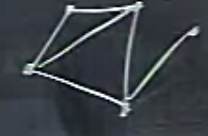
\includegraphics[height=4cm]{11_1.png}

Bu çiziti $5 \times 6$ boyutundaki bir matris ile tarif edebilirim. 

Bir başka örnek, diyelim ki şu anda bu odada olan herkes bir düğüm. Eğer bu
odadaki iki kişi birbiri ile arkadaş ise aralarında bir kenar var
diyelim. Bu sınıf için böyle bir çizit var. Bir diğer çizit ülkenin
tamamındaki insanlar için olabilir, yani 260 milyon düğüm var, ve
arkadaşlığı temsil eden kenarlar. Bu çizite bakıp sorulabilecek ilginç bir
soru şu, herhangi bir düğümden herhangi bir diğer düğüme zıplamak kaç
adımda yapılabilir? Mesela birbirinden en uzak iki insan arasındaki adım
kaç olabilir? Yani.. bir örnek vereyim şimdi, mesela benim ile [o zamanın
ABD başkanı] Bill Clinton arasındaki uzaklık 2. Bir üniversite arkadaşım
Clinton'u tanıyor, böylece mesafemiz 2. Ben şahsen kendisini tanımıyorum,
o yüzden uzaklığım 1 değil, ama ortak bir arkadaşımız var. 

Peki [sınıfa soruyor] sizin Clinton'a uzaklığınız ne? [Cevap 3 diye
geliyor]. Evet tabii, en fazla üç, çünkü siz şimdi beni tanıyorsunuz, sizin
Clinton'a olan uzaklığınızı düşürmekle övünebilirim belki [sınıf
gülüyor]. Peki Monica Lewinsky'ye olan uzaklığınız ne [daha fazla gülüşme],
4'ten daha ufak bir sayı verenin başı dertte :) 

Şaka bir yana, tüm koca çiziti düşünürsek, insanların arasındaki en fazla
uzaklık ne olabilir? Kabaca bu uzaklığın 6 olduğu biliniyor. 6 Derece
Uzaklık (Six Degrees of Seperation) diye bir kitap var mesela, bu başlıklı
bir film de var, ki bahsettikleri konu bu işte. Ve bu sayı pek mantıksız
değil, yani, mesela uçak yolculuğu sırasında biriyle tanışıyorsunuz, sohbet
ederken tanıdıklardan filan bahsediyorsunuz, ve çoğunlukla keşfediyorsunuz
ki aranızda 3-4 basamak var, hatta bazen daha az, sonra ikiniz de ``dünya
ne kadar küçük yahu'' diyorsunuz, ki zaten üstteki çizitin ismi de buradan
geliyor.

İlginç nokta şu, ki bu konuyu daha detaylı bir şekilde sonraki derste
işleyeceğiz; bu çizitte düğümden düğüme giderken birkaç kestirme yol
sayesinde uzaklıklar müthiş bir şekilde azalabiliyor. İşte gördük ki Lineer
Cebir dersimi almakla Clinton'a olan uzaklığınız hemen 3'e düştü
[gülüşmeler]. Tabii matematiksel olarak düşünelim, bu çizitleri bu şekilde
özel yapan nedir? Hatta Web'i düşünürsek, ki sayfaları düğümler, sayfa
arasındaki bağlantıları kenarlar olarak düşünürsek, bu çizitlerin özelliği
nedir? Pek çok kişi bu ağ yapısını anlamak için uğraşıyor. 

Kaynaklar

[1] Bayramlı, Lineer Cebir, {\em Euler Eşitliği, Ders 11} 




\end{document}
